As a baseline we deploy a vanilla OpenDataCam setup using its built-in tools for object counting and path recording.
From the OpenDataCam GUI it's possible to visually inspect the detected objects and draw line counters 
which keep track of the total number of objects passing the line given a certain areal threshold and approach angle. 
The line counters are bi-directional and segment totals based on the mode of transportation.

\ \\
The baseline will focus on the capabilities of only applying OpenDataCam and its tools. This will mostly be "trafic shares" for 
different paths and directions. 
\\ 
We then go on with further data processing as an extension. The main goal is to have a tool catered to analyzing cyclists, capturing
discrete desire lines (with magnitude) and the ability to "hook into" video material for certain scenarios.

\subsection{Hardware}
The pipeline for our setup is shown below on figure \ref{system}. OpenDataCam uses the Yolo4 weights to localize cyclists and pedestrians.
Processing was executed on an ARM based NVIDIA Jetson Xavier NX (development board) equipped with a 384-core NVIDIA Volta GPU
and 8GB of memmory. 

\raggedbottom
\noindent
\begin{tabular}{@{}cc}
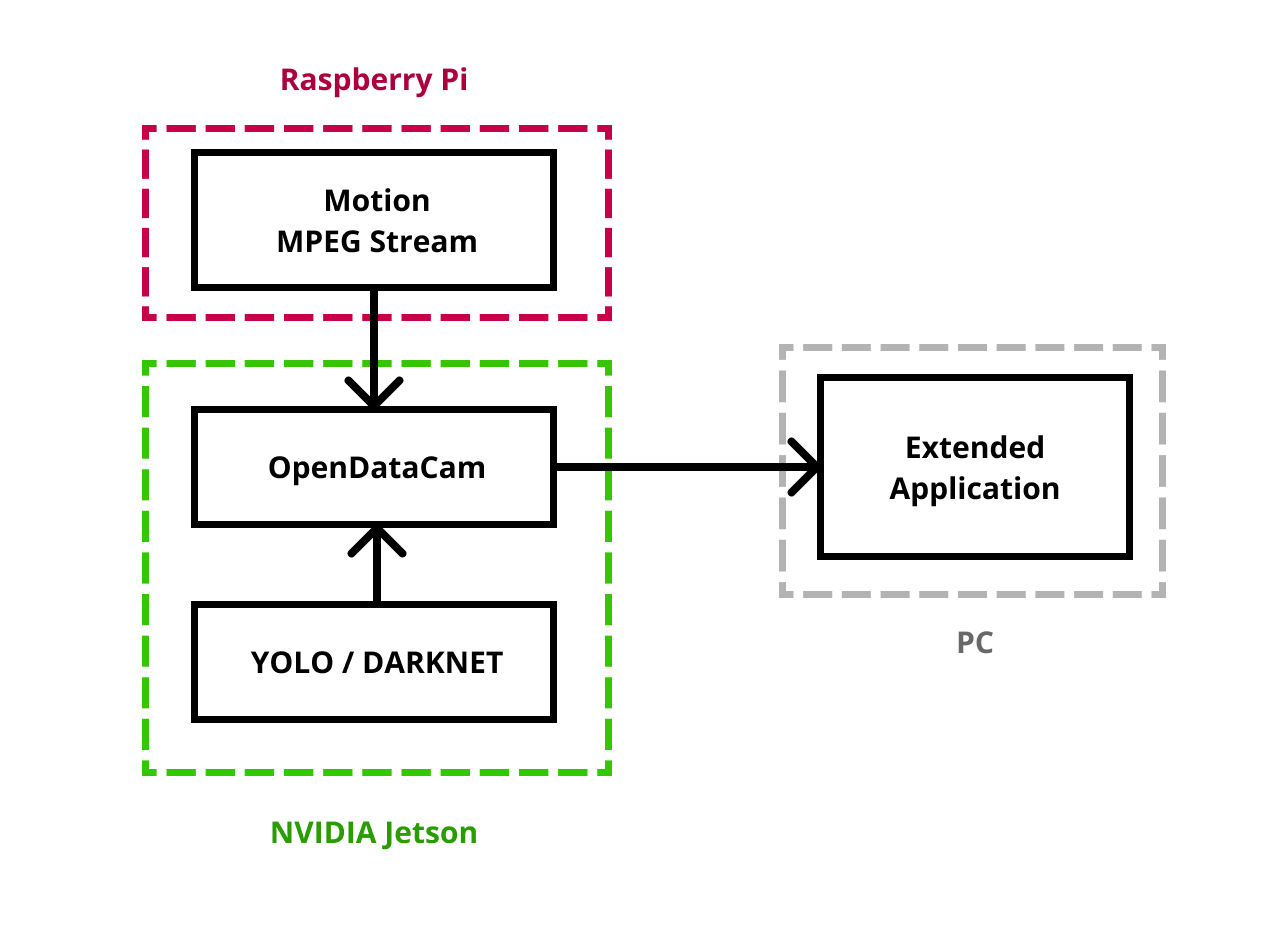
\includegraphics[width=1.0\columnwidth]{system} 
\end{tabular}
\captionof{figure}{System overview}
\label{system}

\ \\
The video feed for YOLO is provided through the OpenDataCam interface, which allows for real-time analysis through an onboard camera
or a video stream from an IP camera. 

\ \\
For further analysis the raw data from the recordings was exported in the form of CSV and JSON files. This includes both the low-level
object detection (bounding-boxes, frame reference, confidence levels etc.) and the totals from the line counters.

\subsection{Case study}
The Dybbølsbro intersection in Copenhagen was chosen as the location for our primary data collection. 
The Dybbølsbro intersection faces several traffic flow challenges as a result development in the immediate vicinity as well as being a large intersection.
These challenges make the Dybbølsbro intersection one of the more extreme in Copenhagen and would serve as a good base to this quantitative analysis method. 

To determine the desire paths that cyclist take throughout the Dybbelsbro intersection we recorded XX hours of footage 
at the Dybbølsbro intersection from X different camera angles.
The considerations taken in choosing a camera angle were:

\begin{itemize}
	\item Camera visibility to cyclists.
	\item Adequate mounting points, in terms of height and surface.
	\item Special attention was also given to making sure that cameras were not mounted on traffic signage.
\end{itemize}

\subsection{Trajectory projection}
The video footage was analyzed using OpenDataCam which is an abstraction layer on top of Yolo. Yolo being an object detection library for object detection in images.
Once the video is analyzed by OpenDataCam, we receive a .json file containing a Unique ID for each identified cyclist that is detected for each frame of the video file. 
The unique ID is accompanied by bounding box coordinates of the detected bicycle on the frame. 
The center-bottom coordinates of the bounding box over multiple frames represents the track of an identified bicycle.

\ \\
By assuming the road as a 2D plane, hereby ignoring any non-linear deformations (e.g. from lens distortion or curvature of the pavement), 
we can transform the pixel positions from the video to real-world 2D coordinates. 
We calculate the \textit{homography matrix}, describing the transformation from one plane to another, by mapping four reference points from each frame (figure \ref{projection_figure}).

\raggedbottom
\ \\ 
\noindent
\begin{tabular}{@{}cc}
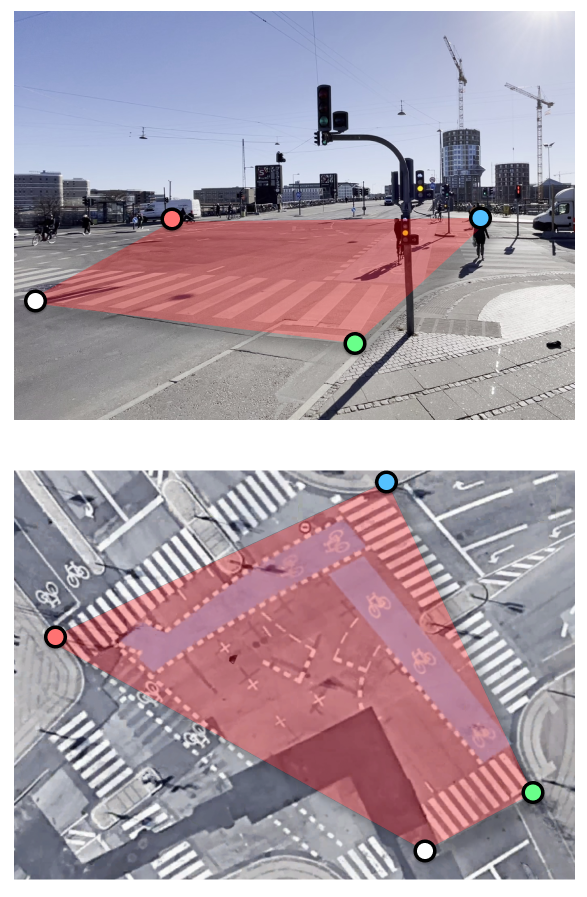
\includegraphics[width=1.0\columnwidth]{projection_figure} 
\end{tabular}
\captionof{figure}{Reference points on map projection}
\label{projection_figure}

\subsection{Trajectory clustering}
Desire Lines

\subsection{Catching unexpected behavior}
"Red zomes" defined by a certain area, speed og trajectory can provide context (through video) when activated. 

